\graphicspath{{members/ssr/figures/}}

\subsection{Greenhouse}\label{subsec:greenhouse}

A greenhouse is a special building for the lone purpose of growing plans under optimal
conditions. It‘s build of (semi)transparent walls and a roof - depending on the specific
needs of the crops and the location.
Environmental controls govern the atmosphere - ideally - for optimal growing conditions.
The controls typically regulate lighting, irrigation and the nutrition provided through
the soil.\\

\begin{figure}[H]
    \centering
    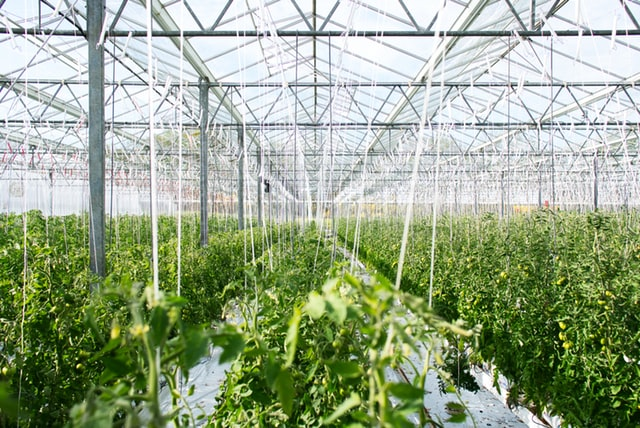
\includegraphics[width=0.8\textwidth]{user-view/greeenhouse_erwan_hesry_unsplash.jpg}
    \caption{Inside a greenhouse}
\end{figure}

Only crops with similar or same optimal growing conditions are grown within each greenhouse unit
since different crops have difference optimal growing conditions in terms of temperature,
humidity, lighting, nutrition etc.\\

\subsubsection*{Layout}

The greenhouse's layout is arranged in ways to optimally make use of the available space by densely
arranging the crops.
Since most greenhouses are used for commercial purposes and in this setting the yield per ground
unit is pivotal, hence the goal is to maximize the yield of each plant.

\begin{figure}[H]
    \centering
    \begin{minipage}[b]{0.47\textwidth}
        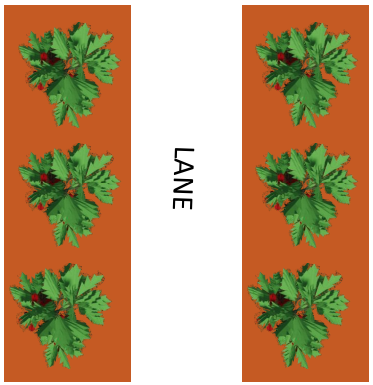
\includegraphics[width=\textwidth]{user-view/lanes.png}
        \caption{Crops arranged in lanes}
    \end{minipage}
    \hfill
    \begin{minipage}[b]{0.49\textwidth}
        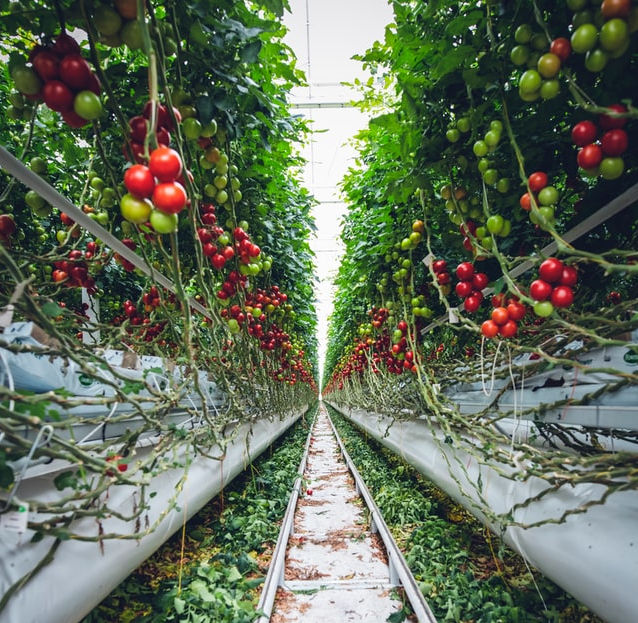
\includegraphics[width=\textwidth]{user-view/plant1_markus_spiske_unsplash.jpg}
        \caption{Walkable lanes}
    \end{minipage}
\end{figure}

\subsubsection*{Lighting}

One central aspect throughout this project is lighting and illumination.
The primary source for bio-activity in plants is photosynthetic active radiation (PAR) -
beside the already mentioned factors. 

\subsection{Plants}\label{subsec:plants}

This section will give a brief overview the plants properties which this project is concerned with.

\subsubsection*{Growth Stages}

Figure \ref{growth-stages} shows the different stages of tomato plant throughout its lifetime.
The relevant features for our purpose here are the plant's geometric development in each growth stage
and the fruit's color change during that time.

\begin{figure}[H]
    \centering
    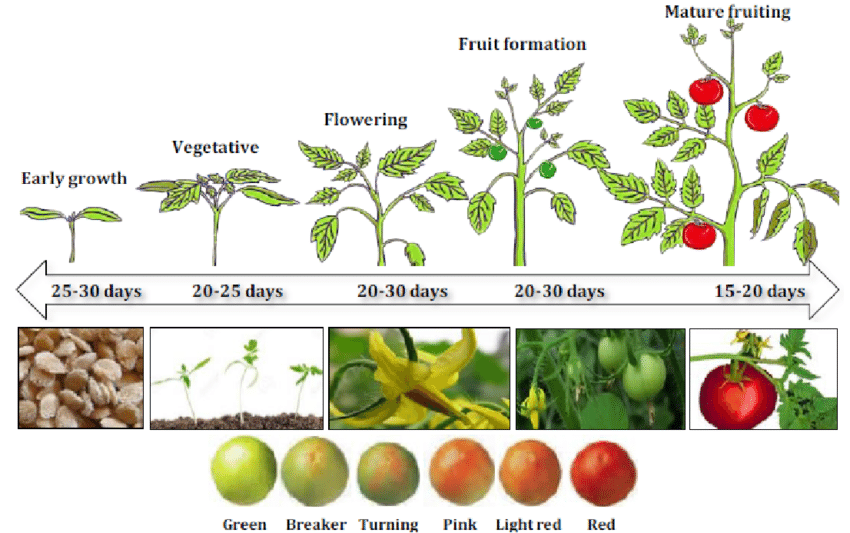
\includegraphics[width=1.0\textwidth]{user-view/growth_stages.png}
    \caption{\enquote{Demonstration of the five growth stages of tomato, and the different levels of fruit ripeness.} \cite{Shamshiri2018}}
    \label{growth-stages}
\end{figure}

Beside other factors each state is basically signified by an increase in branching  and growth, whereby
pre-existing branches grow longer an never mainly appear above existing branches creating multiple levels
of branches with shrinking branch length. 
\newpage
\subsubsection*{Leaf Properties}

The main driver for bio-activity in plants is initiated through the leaves surface interaction.
Either through gas exchange of through photosynthetic active radiation through light.

\begin{figure}[H]
    \centering
    \begin{minipage}[b]{0.49\textwidth}
        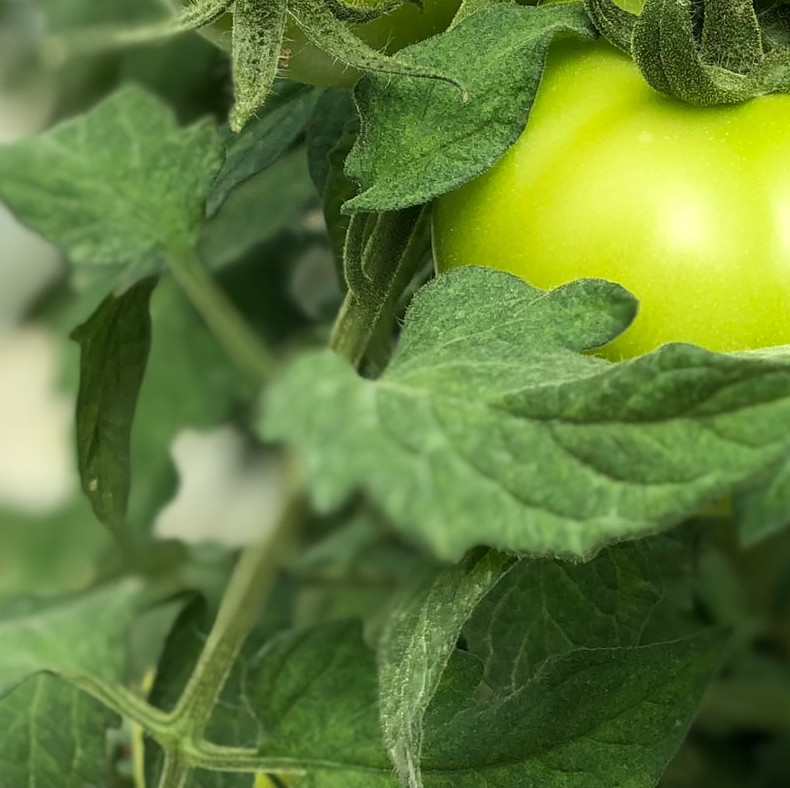
\includegraphics[width=\textwidth]{user-view/plant4_leaf_Soo_Ann_Woon_Unsplash.jpg}
        \caption{Hairy, waxy leaf surface}
    \end{minipage}
    \hfill
    \begin{minipage}[b]{0.49\textwidth}
        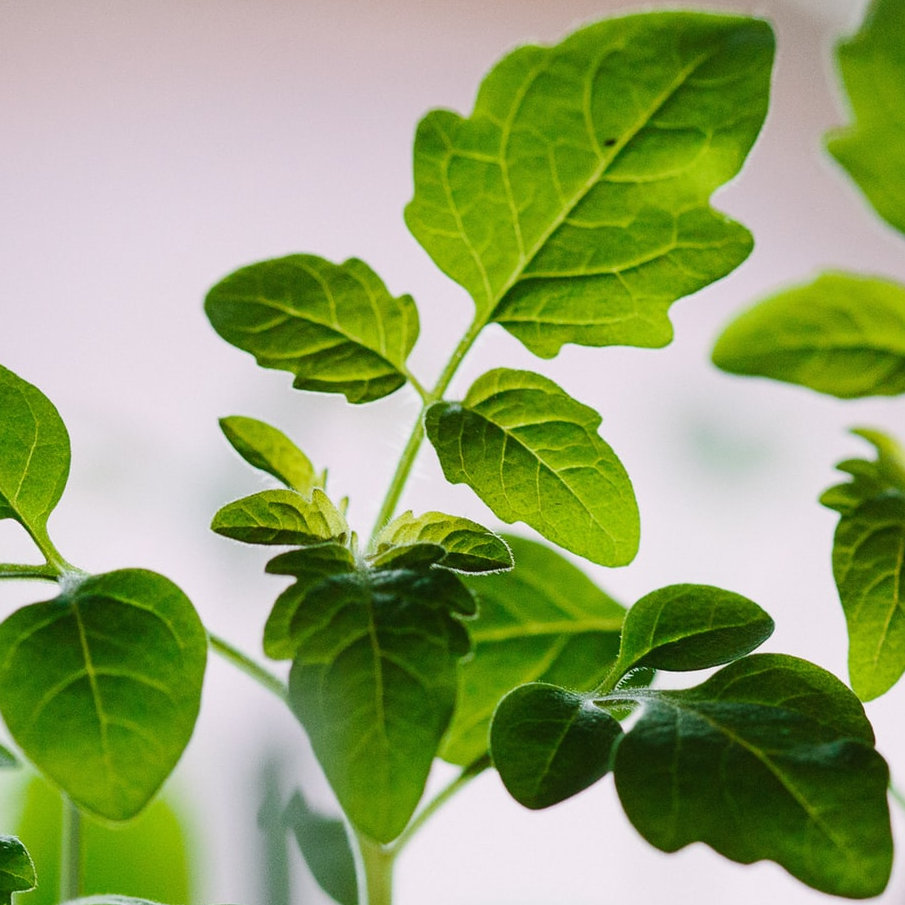
\includegraphics[width=\textwidth]{user-view/plant2_Francesco_Gallarotti_unsplash.jpg}
        \caption{Young leaves partly translucent}
    \end{minipage}
\end{figure}
\newpage
\subsubsection*{Defective Plants}

Defects are either apparent through visibly damaged leaves, fruits or both.
Since these plants have defects their either have impaired or none fruit production.

Figure \ref{fig:septoria} and \ref{fig:blight} show the two most common diseases which are visible through leave changes and
figure \ref{fig:Anthracnose} and \ref{fig:blossom} and show the two most common fruit diseases - both are caused by fungi
and lead to unusable yield \cite{diseases}.

\begin{figure}[H]
    \centering
    \begin{minipage}[b]{0.45\textwidth}
        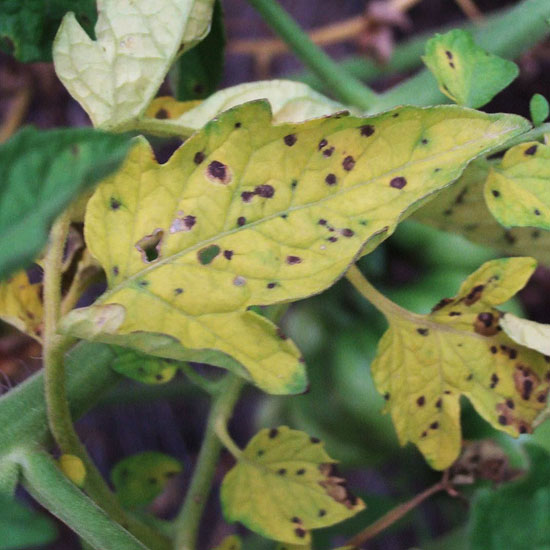
\includegraphics[width=\textwidth]{user-view/sick_0.jpg}
        \caption{Septoria Leaf Spot: Fungus}
        \label{fig:septoria}
    \end{minipage}
    \hfill
    \begin{minipage}[b]{0.45\textwidth}
        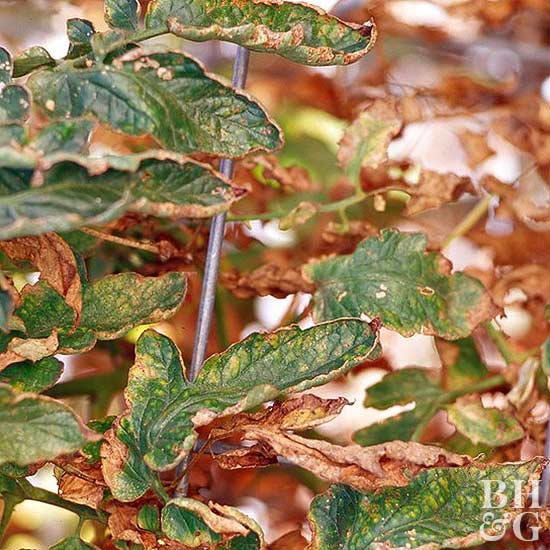
\includegraphics[width=\textwidth]{user-view/sick_1.jpg}
        \caption{Early Blight: Fungus}
        \label{fig:blight}
    \end{minipage}
\end{figure}

As visible the fungi affect leaf surface and color. Both have deviating color and texture
as expected from green healthy leaves.

\begin{figure}[H]
    \centering
    \begin{minipage}[b]{0.45\textwidth}
        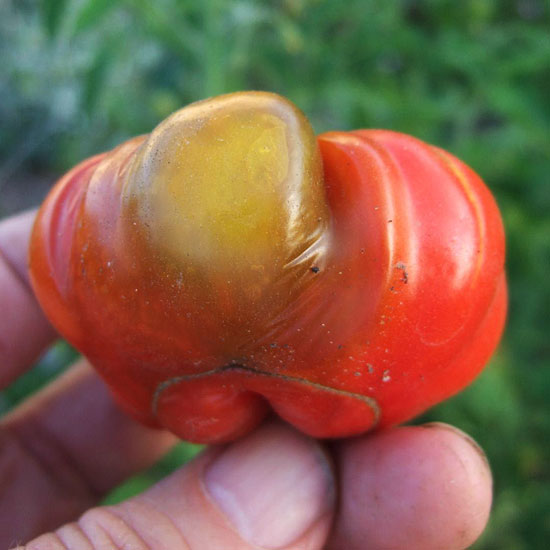
\includegraphics[width=\textwidth]{user-view/sick_2.jpg}
        \caption{Anthracnose: Fungus}
        \label{fig:Anthracnose}
    \end{minipage}
    \hfill
    \begin{minipage}[b]{0.45\textwidth}
        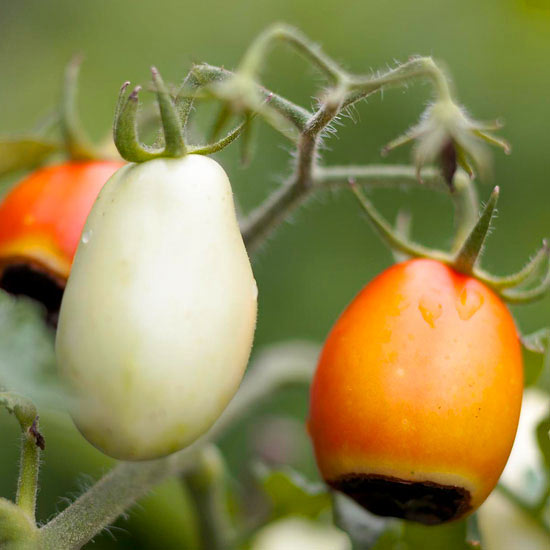
\includegraphics[width=\textwidth]{user-view/sick_3.jpg}
        \caption{Blossom-End Rot}
        \label{fig:blossom}
    \end{minipage}
\end{figure}

This also applies to fruits which have deviating colors as it is expected in the
growing state (yewllow-like color) or have colorings which is not expected in any stage (black rot).

\subsection{Task Requirements}\label{subsec:task-requirements}

This project is concerned with the commercial domain of yield production and its purpose
is to estimate the expected yield.
Hence the goal is to design a solution which can automatically estimate yield based on photo camera images
taken from the greenhouse tomato plants.\\

For this purpose obvious requirements are:
\begin{enumerate}
    \item a reasonable and affordable solution which makes sense from cost and labor perspective
    \item the greenhouse space should be used as effective as possible, means that the number of plants per group unit should be dense
\end{enumerate}
\newpage
